% !TeX program = pdflatex
%==============================================================================
%  Aula 04 --- Métodos Não Paramétricos (KNN)
%  VERSÃO DO ALUNO: texto para leitura autônoma, fora da sala.
%  (O roteiro de sala correspondente é "04 Metodos Nao Parametricos KNN.tex".)
%==============================================================================
\documentclass[11pt,a4paper]{article}
\usepackage[aluno]{../../recursos/latex/estilo-notas}

\title{}
\date{}

\begin{document}
\cabecalhoaula{04}{Métodos Não Paramétricos (KNN)}{AME §4.1--4.5; ISLP §3.5 e cap.~7}

%==============================================================================
\section*{O que você vai aprender}
%==============================================================================
Ao final desta aula você deve ser capaz de:
\begin{itemize}[leftmargin=1.4cm]
  \item explicar o que distingue um método \emph{não paramétrico} de um
        paramétrico e por que ele troca viés por variância;
  \item descrever a estratégia de \emph{bases} (séries ortogonais, \emph{splines})
        para flexibilizar a regressão linear;
  \item definir o estimador de \textbf{$k$ vizinhos mais próximos} (KNN) e o papel
        de $k$ no balanço viés--variância;
  \item definir o estimador de \textbf{Nadaraya--Watson} e reconhecer os
        principais \emph{kernels} de suavização e o papel da janela $h$;
  \item entender a \textbf{regressão polinomial local} como extensão de
        Nadaraya--Watson e sua vantagem na fronteira;
  \item enxergar todos esses métodos como \emph{médias locais} / \emph{suavizadores
        lineares}.
\end{itemize}

\noindent
Esta aula é uma mudança de paradigma em relação às Aulas~01--02. Lá fixávamos a
forma de $r$ --- linear, polinomial de grau $p$ --- e estimávamos poucos parâmetros.
Von Neumann resumiu o desconforto dessa postura numa frase famosa: \emph{``com
quatro parâmetros eu ajusto um elefante; com cinco, faço a tromba mexer.''} A
pergunta desta aula é a consequência natural:

\begin{center}\itshape
  e se eu não quiser supor forma alguma para $r(\x)$?
\end{center}

\noindent
A resposta é deixar os \emph{dados} ditarem a forma. O preço, você já sabe qual é
--- e a Aula~05 vai mostrar que ele é bem mais alto do que parece quando $d$ cresce.

%==============================================================================
\section{O que é um método não paramétrico?}
%==============================================================================
Um método \textbf{paramétrico} supõe que $r(\x)=\E[Y\mid\X=\x]$ pertence a uma
família indexada por um número \emph{fixo e finito} de parâmetros (ex.: regressão
linear, $d+1$ coeficientes). Um método \textbf{não paramétrico} não impõe uma
forma funcional fixa: a complexidade efetiva do modelo \emph{cresce com $n$}. A
suposição é mais fraca --- tipicamente apenas que $r$ é \emph{suave}.

\begin{atencao}[``não paramétrico'' não quer dizer ``sem parâmetros'']
O nome engana. O KNN guarda a base de treino inteira --- em certo sentido, tem
\emph{mais} parâmetros que uma regressão linear, não menos. O que caracteriza o
método é que o número de graus de liberdade \emph{não é fixado de antemão}: ele
acompanha $n$. Com 50 pontos você tem um modelo; com 50 mil, outro, mais rico.
\end{atencao}

\begin{ideia}
Em relação aos paramétricos, métodos não paramétricos \textbf{reduzem o viés}
(capturam relações arbitrárias) ao custo de \textbf{aumentar a variância}.
Continuamos no mundo da Aula~01: o segredo é controlar a flexibilidade por um
\emph{tuning parameter} (o $k$ do KNN, a janela $h$ do kernel), escolhido por
validação cruzada (Aula~03).
\end{ideia}

\begin{observacao}
Há uma ponte importante com a Aula~02. Penalizar um modelo muito flexível (Ridge,
Lasso) e usar um modelo não paramétrico são duas formas de se posicionar no mesmo
balanço viés--variância, vindas de lados opostos: a penalização \emph{aproxima} um
modelo flexível de um simples; o não paramétrico \emph{parte} do flexível e só o
segura o quanto for preciso.
\end{observacao}

%==============================================================================
\section{Estratégia de bases: séries ortogonais e \emph{splines}}
%==============================================================================
A primeira ideia para ganhar flexibilidade sem sair do arcabouço linear é
\textbf{ampliar o conjunto de atributos} com funções $\phi_1,\dots,\phi_I$ das
covariáveis e ajustar
\[
  g(x) = \sum_{j=1}^{I} \beta_j \,\phi_j(x),
\]
que é \emph{linear nos $\beta_j$} --- estimável por mínimos quadrados (Aula~02).
Aqui a flexibilidade é controlada por $I$ (número de funções da base).

\subsection{Séries ortogonais}
Usa-se uma base ortonormal de $L^2$ (Fourier, polinômios ortogonais, \emph{wavelets}).
Aproxima-se $r$ por suas primeiras $I$ componentes na base; $I$ é o \emph{tuning
parameter} (mais termos $\Rightarrow$ mais flexível). É a ideia por trás de
``regressão polinomial'' vista na Aula~01 (a base dos monômios $1,x,x^2,\dots$).

\subsection{\emph{Splines}}
\emph{Splines} são funções polinomiais por partes, ``coladas'' suavemente em
pontos chamados \textbf{nós} (\emph{knots}) $t_1,\dots,t_p$. Uma base conveniente
para \emph{splines} de grau $k$ é
\[
  f_1(x)=1,\ f_2(x)=x,\ \dots,\ f_{k+1}(x)=x^k,\qquad
  f_{k+1+j}(x)=(x-t_j)_+^{k},\ j=1,\dots,p,
\]
onde $(u)_+=\max(u,0)$. Com isso $I=k+1+p$, e novamente estimam-se os
coeficientes por mínimos quadrados.

\begin{ideia}[por que a base truncada funciona]
Vale entender por que $(x-t_j)_+^k$ é a peça certa. Essa função é identicamente
nula à esquerda de $t_j$ e um polinômio de grau $k$ à direita. Somá-la ao modelo,
portanto, \emph{não muda nada antes do nó} e permite mudar a curvatura
\emph{depois} dele --- e como ela e suas $k-1$ primeiras derivadas se anulam em
$t_j$, a emenda sai suave de graça. Cada nó compra exatamente um grau de liberdade
a mais, localizado onde você quiser.
\end{ideia}

\noindent Variantes importantes: \emph{B-splines} (base numericamente estável, é o
que as bibliotecas usam de fato), \emph{natural splines} (impõem linearidade fora
dos nós extremos, reduzindo a variância na fronteira --- mesma preocupação da
Seção~\ref{sec:local}) e \emph{smoothing splines} (em vez de escolher nós, põem um
nó em cada observação e penalizam a curvatura $\int (g''(x))^2dx$ --- caso
particular de RKHS, §4.6 do [AME]).

Poucos nós dão uma curva rígida (subajuste); muitos nós dão uma curva nervosa
(superajuste). O número e a posição dos nós são o botão de complexidade --- é a
Aula~01 de novo, com outro nome.

%==============================================================================
\section{$k$ vizinhos mais próximos (KNN)}
%==============================================================================
O KNN é talvez o método não paramétrico mais intuitivo: para prever em $\x$, faça
a \emph{média das respostas dos $k$ pontos de treino mais próximos de $\x$}.

\begin{definicao}[Regressão KNN]
Seja $\mathcal{N}_{\x}$ o conjunto dos índices das $k$ observações de treino mais
próximas de $\x$ (segundo uma distância $d$, em geral euclidiana):
$\mathcal{N}_{\x}=\{i : d(\X_i,\x)\le d^{k}_{\x}\}$, onde $d^k_{\x}$ é a distância
do $k$-ésimo vizinho. Então
\begin{equation}\label{eq:knn}
  \widehat{r}(\x) = \frac{1}{k}\sum_{i\in\mathcal{N}_{\x}} Y_i .
\end{equation}
\end{definicao}

Repare no que essa fórmula \emph{não} tem: nenhum parâmetro a estimar, nenhuma
otimização, nenhum ajuste. O ``treino'' do KNN consiste em guardar os dados. Todo o
trabalho acontece na hora da predição --- por isso o método é chamado de
\emph{preguiçoso} (\emph{lazy learner}).

O parâmetro $k$ controla a flexibilidade:
\begin{itemize}[leftmargin=1.4cm]
  \item \textbf{$k$ pequeno} (ex.: $k=1$): vizinhança minúscula, segue cada ponto
        $\Rightarrow$ \emph{viés baixo, variância alta} (curva ``nervosa'',
        superajuste).
  \item \textbf{$k$ grande}: média sobre muitos pontos; quando $k\to n$, $\rhat$
        tende à média global (constante) $\Rightarrow$ \emph{viés alto, variância
        baixa} (subajuste).
\end{itemize}
Escolhe-se $k$ por validação cruzada.

\begin{figure}[htbp]
  \centering
  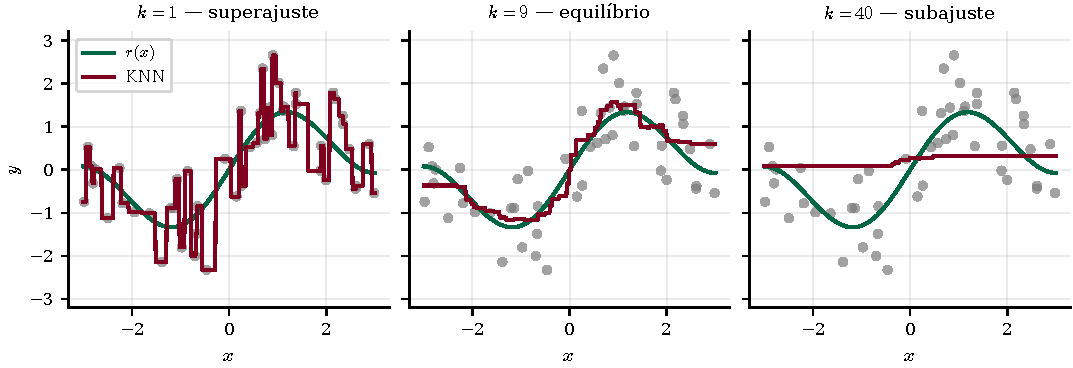
\includegraphics[width=\textwidth]{../../recursos/figuras/04-knn-k.pdf}
  \caption{KNN sobre a mesma amostra de $n=50$ pontos da Aula~01. Com $k=1$ a
  estimativa passa por cima de cada observação e vira uma escada --- é a versão KNN
  do polinômio de grau~15. Com $k=40$, quase toda a amostra entra em cada média e a
  curva quase não distingue um $x$ do outro. O $k$ faz exatamente o papel que o grau
  do polinômio fazia, só que \emph{ao contrário}: aqui é o $k$ \emph{pequeno} que
  significa flexível.}
  \label{fig:knnk}
\end{figure}

\begin{atencao}
KNN exige uma noção de distância e, portanto, \textbf{depende fortemente da escala}
das covariáveis. Se uma variável está em reais e outra em milhares de reais, a
segunda domina completamente a distância euclidiana e a primeira poderia nem existir.
\emph{Padronize} antes (Aula~07). Além disso, o KNN sofre da \emph{maldição da
dimensionalidade}: em $d$ alto, ``vizinhos'' deixam de ser próximos --- é o tema
inteiro da Aula~05.
\end{atencao}

%==============================================================================
\section{Nadaraya--Watson (regressão por kernel)}
%==============================================================================
O KNN dá peso $1/k$ aos $k$ vizinhos e $0$ aos demais --- uma transição abrupta.
Nadaraya--Watson suaviza isso: usa uma \textbf{média ponderada} de \emph{todas} as
observações, com pesos que decaem com a distância.
\begin{equation}\label{eq:nw}
  \widehat{r}(\x) = \sum_{i=1}^n w_i(\x)\,Y_i,
  \qquad
  w_i(\x) = \frac{K(\x,\X_i)}{\sum_{j=1}^n K(\x,\X_j)},
\end{equation}
onde $K$ é um \textbf{kernel de suavização} que mede a similaridade entre $\x$ e
$\X_i$. Note $\sum_i w_i(\x)=1$. Escolhas comuns (com janela/largura $h>0$):
\begin{center}\small
\renewcommand{\arraystretch}{1.4}
\begin{tabular}{@{}ll@{}}
\toprule
\textbf{Kernel} & \textbf{$K(\x,\X_i)$} \\
\midrule
Uniforme       & $\1{d(\x,\X_i)\le h}$ \\
Gaussiano      & $(2\pi h^2)^{-1/2}\exp\!\big(-d^2(\x,\X_i)/(2h^2)\big)$ \\
Triangular     & $\big(1-d(\x,\X_i)/h\big)\,\1{d(\x,\X_i)\le h}$ \\
Epanechnikov   & $\big(1-d^2(\x,\X_i)/h^2\big)\,\1{d(\x,\X_i)\le h}$ \\
\bottomrule
\end{tabular}
\end{center}
O kernel uniforme dá peso igual a todos dentro do raio $h$ (e zero fora); os demais
ponderam pela proximidade; o gaussiano dá peso positivo a todos. A janela $h$ é o
\emph{tuning parameter}: $h$ grande $\Rightarrow$ muita suavização (viés alto,
variância baixa); $h$ pequeno $\Rightarrow$ pouca (variância alta, viés baixo).

\begin{figure}[htbp]
  \centering
  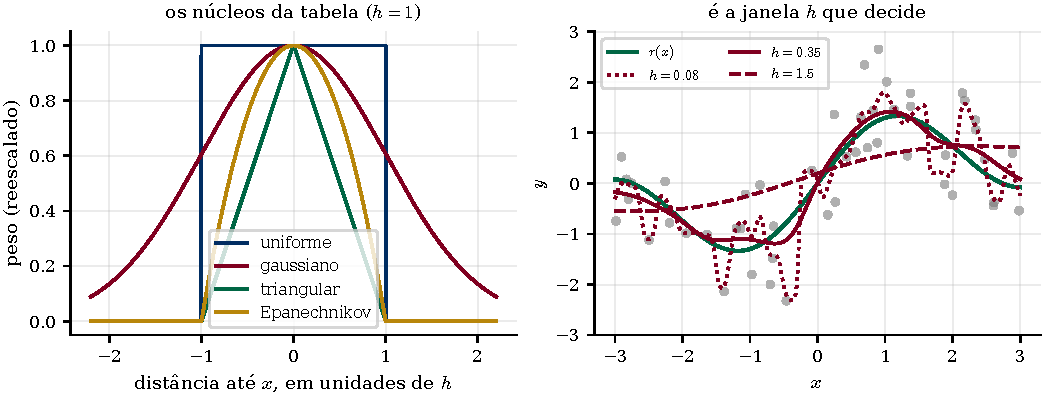
\includegraphics[width=\textwidth]{../../recursos/figuras/04-nucleos.pdf}
  \caption{À esquerda, os quatro núcleos da tabela, todos com $h=1$ e reescalados
  para topo $1$: eles diferem no formato, mas todos fazem a mesma coisa --- dar mais
  peso a quem está perto. À direita, o que \emph{de fato} muda o ajuste: com o mesmo
  núcleo gaussiano, $h=0{,}08$ persegue o ruído, $h=1{,}5$ achata a senoide até quase
  uma reta, e $h=0{,}35$ acerta.}
  \label{fig:nucleos}
\end{figure}

\begin{observacao}[Na prática, a janela importa mais que o kernel]
Empiricamente, a escolha do \emph{kernel} pouco afeta o resultado; o que importa é
o \emph{tuning parameter} $h$ (ou $k$). A Figura~\ref{fig:nucleos} explica por quê:
os quatro núcleos são versões ligeiramente diferentes do mesmo perfil, enquanto
mudar $h$ altera a \emph{escala} da vizinhança em ordens de grandeza. Foque a
validação cruzada em $h$ e não perca tempo comparando núcleos.
\end{observacao}

\subsection{Nadaraya--Watson como mínimos quadrados ponderados locais}
Há uma leitura iluminadora: $\widehat r(\x)$ em \eqref{eq:nw} é o intercepto
$\widehat\beta_0$ que resolve
\begin{equation}\label{eq:nwls}
  \widehat\beta_0 = \argmin_{\beta_0}\sum_{i=1}^n w_i(\x)\,(Y_i-\beta_0)^2 .
\end{equation}
Ou seja: \emph{em cada ponto $\x$}, ajustamos uma \textbf{constante} por mínimos
quadrados, ponderando as observações pela proximidade a $\x$. É um ajuste linear
\emph{local}.

\begin{proof}
Derivando \eqref{eq:nwls} em $\beta_0$ e igualando a zero:
$-2\sum_i w_i(\x)(Y_i-\beta_0)=0 \Rightarrow \beta_0
=\frac{\sum_i w_i(\x)Y_i}{\sum_i w_i(\x)}=\sum_i w_i(\x)Y_i$, pois os pesos somam
$1$. Logo $\widehat\beta_0$ coincide com \eqref{eq:nw}.
\end{proof}

\begin{ideia}
Essa releitura é mais do que uma curiosidade: ela abre a porta da próxima seção. Se
ajustar uma \emph{constante} localmente já dá um método útil, nada impede ajustar
uma \emph{reta}, ou uma parábola. É a mesma equação com mais termos.
\end{ideia}

%==============================================================================
\section{Regressão polinomial local}\label{sec:local}
%==============================================================================
A regressão polinomial local (LOESS/LOWESS) substitui o intercepto por um polinômio
de grau $p$:
\begin{equation}\label{eq:loess}
  \widehat\beta_0,\dots,\widehat\beta_p
   = \argmin_{\beta_0,\dots,\beta_p}\sum_{i=1}^n w_i(\x)
     \Big(Y_i - \beta_0 - \textstyle\sum_{j=1}^p \beta_j x_i^{\,j}\Big)^2,
\end{equation}
e a predição em $\x$ é $\widehat\beta_0$. Em forma matricial, com $\bm{B}$ tendo
$i$-ésima linha $(1,x_i,\dots,x_i^p)$ e $\bm{\Omega}=\operatorname{diag}(w_i(\x))$:
\[
  (\widehat\beta_0,\dots,\widehat\beta_p)^\top
   = (\bm{B}^\top\bm{\Omega}\bm{B})^{-1}\bm{B}^\top\bm{\Omega}\,\bm{Y}.
\]
Para \emph{cada} $\x$ resolve-se um problema diferente (os pesos mudam). Tomando
$p=0$ recupera-se Nadaraya--Watson.

\subsection{O problema da fronteira}
A vantagem do grau $p\ge 1$ aparece nas \emph{bordas} do domínio, e vale entender
o mecanismo. Tome $\x$ na ponta direita do suporte. A vizinhança de $\x$ só tem
pontos \emph{de um lado} --- todos à esquerda. Se $r$ está subindo ali, a média
local desses pontos é uma média de valores \emph{menores} que $r(\x)$, e a
estimativa fica sistematicamente puxada para baixo. Não é ruído: é viés, e ele não
desaparece por mais dados que você colete.

A reta local não cai nessa armadilha porque ela \emph{estima a inclinação} e
extrapola com ela. A Figura~\ref{fig:fronteira} mede o efeito.

\begin{figure}[htbp]
  \centering
  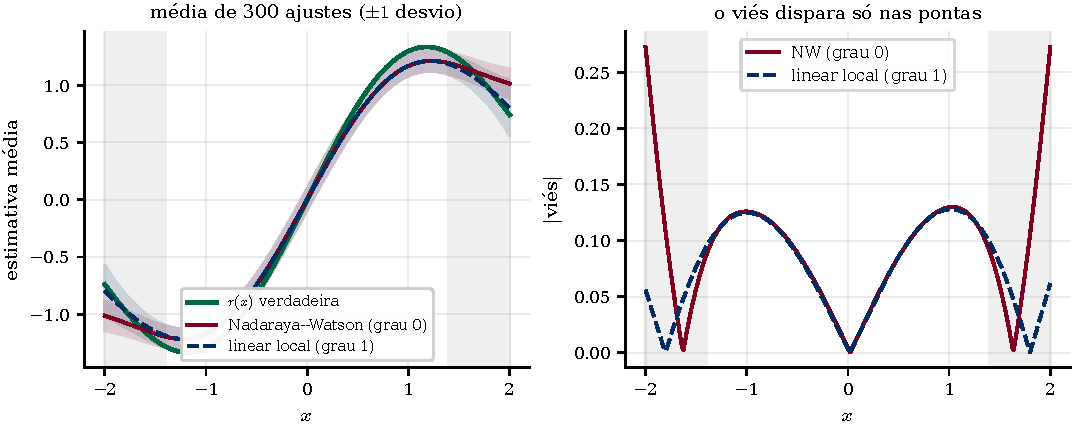
\includegraphics[width=\textwidth]{../../recursos/figuras/04-fronteira.pdf}
  \caption{Viés medido em 300 amostras independentes ($n=200$, $h=0{,}35$, núcleo
  gaussiano). À esquerda, a estimativa \emph{média} de cada método com uma faixa de
  $\pm1$ desvio-padrão: no miolo as duas acompanham $r$, mas nas pontas a curva do
  Nadaraya--Watson descola. À direita, o mesmo em números: o viés é idêntico nos dois
  métodos ao longo de todo o interior e \emph{dispara} apenas nas faixas cinza. Em
  média sobre a fronteira, o viés cai de $0{,}097$ (grau 0) para $0{,}045$ (grau 1)
  --- menos da metade.}
  \label{fig:fronteira}
\end{figure}

\begin{atencao}[o grau 1 não é de graça]
Na mesma simulação, o desvio-padrão na fronteira \emph{sobe} de $0{,}108$ (grau 0)
para $0{,}138$ (grau 1): estimar uma inclinação a partir de poucos pontos de um lado
só é uma tarefa ruidosa. Você trocou viés por variância outra vez --- e se $n$ for
pequeno, a troca pode não compensar. É a Aula~01, agora dentro de uma janela.
\end{atencao}

%==============================================================================
\section{Uma visão unificadora: suavizadores lineares}
%==============================================================================
KNN, Nadaraya--Watson, \emph{splines} e regressão local são todos
\textbf{suavizadores lineares}: a predição é uma combinação linear das respostas,
\[
  \widehat{r}(\x) = \sum_{i=1}^n \ell_i(\x)\,Y_i,
\]
com pesos $\ell_i(\x)$ que dependem só das covariáveis (não de $\bm{Y}$). Para o
KNN, $\ell_i(\x)=\tfrac1k\1{i\in\mathcal{N}_{\x}}$; para NW, $\ell_i(\x)=w_i(\x)$.

\begin{ideia}
Vista assim, a diferença entre os métodos desta aula é só \emph{o formato dos
pesos}: o KNN usa uma janela retangular de largura variável (larga onde há poucos
dados, estreita onde há muitos); o Nadaraya--Watson, uma janela de largura fixa e
bordas suaves. Essa estrutura comum explica por que todos enfrentam o mesmo dilema
--- largura da vizinhança $\leftrightarrow$ complexidade --- e por que valem para
todos os atalhos vistos antes, como o do LOOCV via \emph{leverage} (Aula~03,
Prop.~3.1): basta que $\ell_i(\x)$ não dependa de $\bm{Y}$.
\end{ideia}

%==============================================================================
\section{Prática em Python}
%==============================================================================
\begin{lstlisting}
from sklearn.neighbors import KNeighborsRegressor
from sklearn.preprocessing import StandardScaler
from sklearn.pipeline import make_pipeline
from sklearn.model_selection import GridSearchCV

# KNN com k escolhido por validacao cruzada (padronizando dentro do pipeline!)
modelo = make_pipeline(StandardScaler(), KNeighborsRegressor())
grade  = {"kneighborsregressor__n_neighbors": [1, 3, 5, 11, 25, 51]}
busca  = GridSearchCV(modelo, grade, cv=5, scoring="neg_mean_squared_error")
busca.fit(X_tr, y_tr)
print("melhor k:", busca.best_params_)
\end{lstlisting}
O \texttt{StandardScaler} dentro do \emph{pipeline} não é preciosismo: sem ele o
KNN mede distâncias em unidades misturadas, e com ele a padronização é refeita
dentro de cada dobra, sem vazamento (Aulas~03 e~07).

Para Nadaraya--Watson e regressão local, \texttt{statsmodels} traz \texttt{lowess} e
\texttt{KernelReg} (em \texttt{statsmodels.nonparametric}). O notebook
\texttt{Aula prática 03, 04 e 05} explora $k$ e $h$ em dados artificiais e no
\texttt{superconductivity.csv}.

%==============================================================================
\section*{Resumo}
%==============================================================================
\begin{itemize}[leftmargin=1.4cm]
  \item Métodos não paramétricos não fixam a forma de $r$; reduzem viés e aumentam
        variância em relação aos paramétricos. A complexidade cresce com $n$.
  \item \emph{Bases} (séries, \emph{splines}): linearizam o problema; flexibilidade
        via número de termos/nós.
  \item \textbf{KNN} \eqref{eq:knn}: média dos $k$ vizinhos; $k$ controla
        viés--variância, com $k$ \emph{pequeno} $=$ flexível
        (Fig.~\ref{fig:knnk}).
  \item \textbf{Nadaraya--Watson} \eqref{eq:nw}: média ponderada por kernel; a
        janela $h$ é o que importa, não o kernel (Fig.~\ref{fig:nucleos}); é uma
        constante ajustada localmente \eqref{eq:nwls}.
  \item \textbf{Regressão polinomial local}: polinômio local; corta o viés de
        fronteira pela metade, ao custo de mais variância lá
        (Fig.~\ref{fig:fronteira}).
  \item Todos são \emph{suavizadores lineares}; \emph{padronize} as covariáveis e
        cuidado com a dimensão (Aula~05).
\end{itemize}

\paragraph{Leitura recomendada.} [AME] §4.1--4.2 (séries e \emph{splines}), §4.3
(KNN, com a Figura~4.2 sobre o efeito de $k$), §4.4 (Nadaraya--Watson, Figuras~4.3
e~4.4 --- esta última compara dois kernels e mostra o quanto isso importa pouco) e
§4.5 (regressão polinomial local). [ISLP] §3.5 (regressão linear $\times$ KNN, onde
fica claro quando o paramétrico ainda ganha) e Capítulo~7 inteiro
(\emph{Moving Beyond Linearity}), em especial §7.4--7.6 sobre \emph{splines} e
regressão local.

\paragraph{Para praticar.} \texttt{recursos/listas/Lista de exercícios 04.pdf}.

\end{document}
